The client asks for a java framework that works on either Android or desktop, to support the connection between a Arduino board and social services.

If a programmer wants to use the framework to connect a social service to the Arduino board, he would like to work with data in either end and forward it.

Example 1:
He would like to retrieve data from the social service, do something with it, and push data to the Arduino.

Example 2:
He would like to grab data from the Arduino, do something with it, and upload it to a social service.

This illustrates a split in the middle where the developer wants to treat the data himself. Since there is no direct connection between a social service and the Arduino board from our framework, it makes sense to split the framework into two parts.

Framework part one: Retrieving and uploading data between social service and java.

Framework part two: Grab and push data between the Arduino board and java.

Both frameworks would need to support Android and development. This is an advantage for us who is going to create the framework, and for those who are going to use it.

It's easier for us to create the framework since

The disadvantage is that it will be no direct connection from the Arduino board to a social service.
I.e, the board can not connect directly through the Internet to Facebook. It needs a middleman, either a Android phone or a laptop.



After some tests, we have figured out that it makes no difference if the Arduino board is connected through a Bluetooth device or trough an USB cable. If it's an USB cable, the board shows up as a COM port. If the board is paired with the computer/mobile using the operating system/Android, it also shows up as a COM port. So the program searches the COM ports and connects to the board anyhow. (It's may not work on all bluetooth chipsets)


The board needs a firmware that is precompiled on a computer.
That process should be easy for the developer.

\begin{figure}
	\centering
	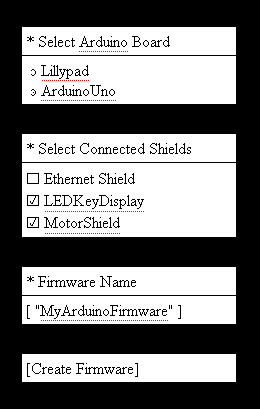
\includegraphics{./img/architecture-mockupgui.png}
	\caption{An early mockup of the GUI}
	\label{fig:architecture-mockupgui}
\end{figure}

On Create Firmware it should be compiled a file that the developer implements in his Arduino program.

\section{Example run framework part 1}

How the developer connects to board on Android/PC after pairing the Arduino with system.

//We search the COM ports trying to find the board
Arduinoboard board = Arduinoboard.findBoard();

//We retrive the current firmware name onboardString currentFirmware = board.getFirmwareName();

if(currentFirmware.equals("MyArduinoFirmware"){
    //Everything is OK, the firmware we want is on board.
}
else{
    //There is wrong Firmware/no firmware
    //We upload the one we precreated on our computer.
    File file = new File("/firmwareLocation/firm.fw");
    ArduinoFirmware fw = ArduinoFirmware.getFW(file);

    board.uploadFirmware(fw);
}

//We can see what shields we have according to the premade firmware
ArduinoShield shields = board.getShields();

//Or we can ask for the shield directly
LEDKeyPadShield display = board.getShield(LEDKeyPadShield.class);

//Now the developer can do what he wants with the shields.
display.printText("HelloWorld");

\section{Overall first design of Arduino – Java Connection}

\begin{figure}
	\centering
	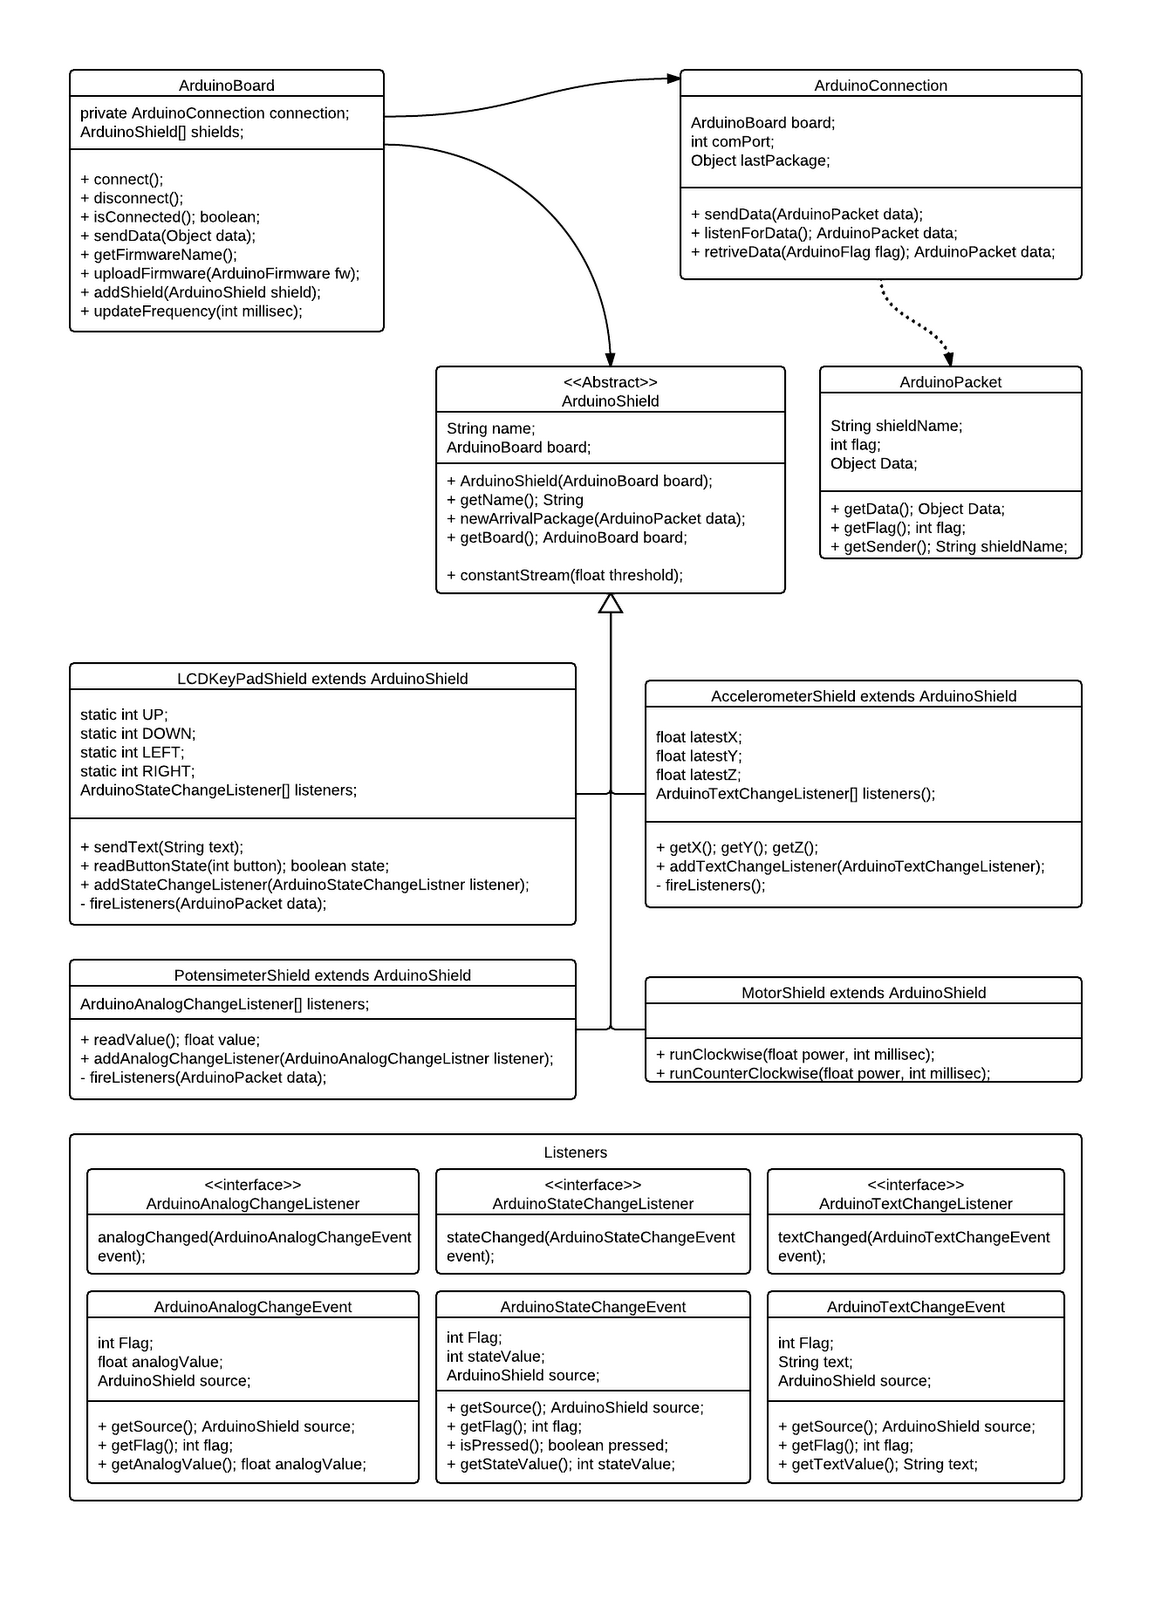
\includegraphics{./img/architecture-arduinojava.png}
	\caption{Conceptual Arduino to Java Connection}
	\label{fig:architecture-arduinojava}
\end{figure}


\section{Adding a listener to shield}


Developer adds his listener.
====
LEDKeyPadShield display = board.getShield(LEDKeyPadShield.class);
display.addStateChangeListener(new ArduinoStateChangeListener(){
  @Override
   public void stateChanged(ArduinoStateChangeEvent event) {
    if(event.getFlag == LEDKeyPadShield.DOWN){
        //Get down and boogie
    }
   }
});
====

In ArduinoConnection we have listenForData(); method, that has its own thread listening on it.

Steps:
listenForData() recives a ArduinoPacked data from Arduino board.

Thread looks in board.shields to find the same board as packet.getName().

It dumps the package into the shield.newArrivalPackage(dataPackage);

It is then up to the shield class to extract the data from package, and fire off an ArduinoEvent to the listeners.

====


\section{Constant data stream solutions}

Some shields, like the accelerometer is sensitive and will always send data to the program. On a mobile phone who constantly needs to work on these packages this will be straining on the battery.

The constantStream threshold value is a signal to the ArduinoBoard to indicate how often in will update.

Threshold = 0.0f; means all data will be streamed
Threshold = 1.0f; means no data will be send from shield to the program. You can only retrieve data by specifically asking for it.

A mid value is dependent on the Shields connected, if the accelerometer has upper values in x,y,z directions from <-1000, 1000>, a threshold of 0.8f indicates we need extreme sudden change of $\Delta(0.8*2000)$ in one of the x,y,z axis to send a notification from the Arduino board.

Example, extremely sudden change (In one cycle?) from -700 to +800 in x direction.  

It's not yet clear if we can implement this function into the firmware.

\section{Example run framework part 2}

//In this case, we register our service with a premade simple Facebook app we have created on
//Facebook.com
SocialService service = new FacebookService(FacebookSevice.getAppAuth("appName"));

//The initateLogin will call up a browser window and request user to log in
//(automatically handle the calls depending if its called from Android or PC)
service.initateLogin();

//Adding listener
service.addSocialListener(new SocialListener(){
  @Override
   public void newPost(Post post) {
    String message = post.message[0];
   }
});

//New post
service.postNewPost(new Post("Hello Profile"));
